\section*{NAIL062 P\&P Logic: Worksheet 4 -- The tableau method}
% after Lecture 4



\subsection*{Teaching goals:} After completing, the student

    \begin{itemize}\setlength{\itemsep}{0pt}
        \item knows terminology of tableau method (entry, tableau, tableau proof/refutation, finished/contradictory branch, canonical model), can define them formally, give examples
        \item knows atomic tableaux, can create suitable atomic tableaux for any logical connective
        \item can construct finished tableau for given proposition from given (even infinite) theory
        \item can describe the canonical model for a given finished noncontradictory branch of a tableau
        \item can apply the tableau method to solve a given problem (word problem, etc.)
        \item knows the compactness theorem and can apply it
    \end{itemize}

    

\section*{In-class problems}


\begin{problem}
    
    Aladdin found two chests in a cave, A and B. He knows that each chest contains either a treasure or a deadly trap. The chests have the following inscriptions:
    \begin{itemize}
    \item On chest A: {\it ``At least one of these two chests contains a treasure.''}
    \item On chest B: {\it ``Chest A contains a deadly trap.''}
    \end{itemize}
    Aladdin knows that either both inscriptions are true, or both are false.
    \begin{enumerate}[(a)]
        \item Express Aladdin's information as a theory $T$ over a suitably chosen set of propositional variables $\mathbb P$. (Explain the meaning of each propositional variable in $\mathbb P$.)
        \item Try to construct tableau proofs from the theory $T$ for the propositions ``The treasure is in chest A'' and ``The treasure is in chest B''.
        \item If any of these finished tableaux is noncontradictory, construct the canonical model for one of its noncontradictory branches.
        \item What conclusion can we draw from this?
    \end{enumerate}

    \begin{solution}
        \begin{enumerate}[(a)]
            \item From the context, we recognize that `either...or' is exclusive (a chest cannot contain both a treasure and a deadly trap). We choose the language $\mathbb P=\{a,b\}$, where $a$ means `chest A contains a treasure', and similarly for $b$. The inscriptions on the chests are formalized as the propositions $a\lor b$ and $\neg a$. The theory $T$ expresses that both are true or both are false:
            $$
            T=\{((a\lor b)\land \neg a)\lor(\neg (a\lor b)\land \neg\neg a)\}
            $$
            (Alternatively, we could formalize it as $T=\{(a\lor b)\liff \neg a\}$, i.e., noticing that ``both true or both false'' means equivalence. The tableau would be slightly smaller but otherwise similar—try it!)
            \item The tableaux have at their root the entries $\mathrm{F}a$ and $\mathrm{F}b$ (we prove by contradiction):
            %\begin{multicols}{2}
                \begin{center}
                    \begin{forest}
                        [$\mathrm{F}a$
                            [$\mathrm{T}((a\lor b)\land \neg a)\lor(\neg (a\lor b)\land \neg\neg a)$
                                [$\mathrm{T}(a\lor b)\land \neg a$
                                    [$\mathrm{T}(a\lor b)$
                                        [$\mathrm{T}\neg a$
                                            [$\mathrm{F}a$
                                                [$\mathrm{T}a$, tikz={\node[fit to=tree,label=below:$\otimes$] {};}]
                                                [$\mathrm{T}b$, tikz={\node[fit to=tree,label=below:$\checkmark$] {};}]
                                            ]
                                        ]
                                    ]                            
                                ]
                                [$\mathrm{T}\neg (a\lor b)\land \neg\neg a$
                                    [$\mathrm{T}\neg (a\lor b)$
                                        [$\mathrm{T}\neg\neg a$
                                            [$\mathrm{F}\neg a$
                                                [$\mathrm{T}a$, tikz={\node[fit to=tree,label=below:$\otimes$] {};}]
                                            ]
                                        ]
                                    ]
                                ]
                            ]                        
                        ]            
                    \end{forest}
                \end{center}                

                \begin{center}
                    \begin{forest}
                        [$\mathrm{F}b$
                            [$\mathrm{T}((a\lor b)\land \neg a)\lor(\neg (a\lor b)\land \neg\neg a)$
                                [$\mathrm{T}(a\lor b)\land \neg a$
                                    [$\mathrm{T}(a\lor b)$
                                        [$\mathrm{T}\neg a$
                                            [$\mathrm{T}a$
                                                [$\mathrm{F}a$, tikz={\node[fit to=tree,label=below:$\otimes$] {};}]
                                            ]
                                            [$\mathrm{T}b$, tikz={\node[fit to=tree,label=below:$\otimes$] {};}]
                                        ]
                                    ]                            
                                ]
                                [$\mathrm{T}\neg (a\lor b)\land \neg\neg a$
                                    [$\mathrm{T}\neg (a\lor b)$
                                        [$\mathrm{T}\neg\neg a$
                                            [$\mathrm{F}a\lor b$
                                                [$\mathrm{F}a$
                                                    [$\mathrm{F}b$
                                                        [$\mathrm{F}\neg a$
                                                            [$\mathrm{T}a$, tikz={\node[fit to=tree,label=below:$\otimes$] {};}]
                                                        ]
                                                    ]
                                                ]
                                            ]
                                        ]
                                    ]
                                ]
                            ]                        
                        ]            
                    \end{forest}
                \end{center}
            %\end{multicols}
            \item The first tableau is finished but noncontradictory. The noncontradictory branch contains the entries $\mathrm{F}a$, $\mathrm{T}b$, and the canonical model for this branch is $v=(0,1)$. It is a model of the theory $T$, in which chest A does not contain a treasure, providing a counterexample to the statement that chest A contains a treasure.
            \item The second tableau is contradictory, so it is a tableau proof and we know that chest B contains the treasure.
        \end{enumerate}

    \end{solution}

\end{problem}


\begin{problem}

    Consider the infinite propositional theory (a) $T=\{p_{i+1} \to p_i\mid i\in \mathbb{N}\}$ (b) $T=\{p_i \to p_{i+1}\mid i\in \mathbb{N}\}$. Using the tableau method, find all models of $T$. Is every model of $T$ a canonical model for some branch of this tableau?

    \begin{solution}

        Construct a tableau from the theory $T$, placing the entry $\mathrm{T}\alpha_0$ at the root, where $\alpha_0$ is the first axiom of $T$. We only show the beginning of the construction; if you need to, construct more.

        First, let us solve (a):
        
        \begin{center}
            \begin{forest}
                [$\mathrm{T}p_1\to p_0$ 
                    [$\mathrm{F}p_1$
                        [$\mathrm{T}p_2\to p_1$ 
                            [$\mathrm{F}p_2$
                                [$\mathrm{T}p_3\to p_2$ 
                                    [$\mathrm{F}p_3$, tikz={\node[fit to=tree,label=below:$\vdots$] {};}]
                                    [$\mathrm{T}p_2$, tikz={\node[fit to=tree,label=below:$\otimes$] {};}]              
                                ] 
                            ]
                            [$\mathrm{T}p_1$, tikz={\node[fit to=tree,label=below:$\otimes$] {};}]              
                        ]
                    ]
                    [$\mathrm{T}p_0$
                        [$\mathrm{T}p_2\to p_1$ 
                            [$\mathrm{F}p_2$
                                [$\mathrm{T}p_3\to p_2$ 
                                    [$\mathrm{F}p_3$, tikz={\node[fit to=tree,label=below:$\vdots$] {};}]
                                    [$\mathrm{T}p_2$, tikz={\node[fit to=tree,label=below:$\otimes$] {};}]         
                                ]
                            ]
                            [$\mathrm{T}p_1$
                                [$\mathrm{T}p_3\to p_2$ 
                                    [$\mathrm{F}p_3$, tikz={\node[fit to=tree,label=below:$\vdots$] {};}]
                                    [$\mathrm{T}p_2$, tikz={\node[fit to=tree,label=below:$\vdots$] {};}]         
                                ]
                            ]              
                        ]
                    ]
                ]
            \end{forest}
        \end{center}
        Each model of $T$ agrees with some (noncontradictory) branch of this (finished) tableau. (Here, in fact, every model of $T$ is a \emph{canonical} model for some branch. In general, this does not necessarily hold.) The models are: $\M(T)=\{v_{<k}\mid k\in\mathbb N\}\cup\{v_\text{all}\}$, where $v_\text{all}(p_i)=1$ for all $i\in\mathbb N$, and
        $$
        v_{<k}(p_i)=\begin{cases}
            1 & \text{ if }i<k,\\
            0 & \text{ if }i\geq k.            
        \end{cases}
        $$
        
        Now (b):

        \begin{center}
            \begin{forest}
                [$\mathrm{T}p_0\to p_1$ 
                    [$\mathrm{F}p_0$
                        [$\mathrm{T}p_1\to p_2$ 
                            [$\mathrm{F}p_1$
                                [$\mathrm{T}p_2\to p_3$ 
                                    [$\mathrm{F}p_2$, tikz={\node[fit to=tree,label=below:$\vdots$] {};}]
                                    [$\mathrm{T}p_3$, tikz={\node[fit to=tree,label=below:$\vdots$] {};}]              
                                ] 
                            ]
                            [$\mathrm{T}p_2$
                                [$\mathrm{T}p_2\to p_3$ 
                                    [$\mathrm{F}p_2$, tikz={\node[fit to=tree,label=below:$\otimes$] {};}]
                                    [$\mathrm{T}p_3$, tikz={\node[fit to=tree,label=below:$\vdots$] {};}]         
                                ]
                            ]              
                        ]
                    ]
                    [$\mathrm{T}p_1$
                        [$\mathrm{T}p_1\to p_2$ 
                            [$\mathrm{F}p_1$, tikz={\node[fit to=tree,label=below:$\otimes$] {};}]         
                            [$\mathrm{T}p_2$
                                [$\mathrm{T}p_2\to p_3$ 
                                    [$\mathrm{F}p_2$, tikz={\node[fit to=tree,label=below:$\otimes$] {};}] 
                                    [$\mathrm{T}p_3$, tikz={\node[fit to=tree,label=below:$\vdots$] {};}]         
                                ]
                            ]              
                        ]
                    ]
                ]
            \end{forest}
        \end{center}

        Again, it is not hard to see that each model agrees with some branch. We have $\M(T)=\{v_\text{none}\}\cup\{v_{\geq k}\mid k\in\mathbb N\}$, where $v_\text{none}(p_i)=0$ for all $i\in\mathbb N$, and
        $$
        v_{\geq k}(p_i)=\begin{cases}
            0 & \text{ if }i<k,\\
            1 & \text{ if }i\geq k.            
        \end{cases}
        $$
                    
    \end{solution}

\end{problem}


\begin{problem}

    Design suitable atomic tableaux for the logical connective $\oplus$ (XOR) and show that if a model satisfies the root of your atomic tableau, it also satisfies some branch.

    \begin{solution}

        We need two atomic tableaux, for entries of the form $\mathrm{T}\varphi\oplus\psi$ and $\mathrm{F}\varphi\oplus\psi$. They can look, for example, as follows; verify the condition yourself (easily semantically):

        \begin{multicols}{2}

            \centering
            \begin{forest}
                [$\mathrm{T}\varphi\oplus\psi$
                    [$\mathrm{T}\varphi$
                        [$\mathrm{F}\psi$]
                    ]
                    [$\mathrm{F}\varphi$
                        [$\mathrm{T}\psi$]
                    ]                        
                ]            
            \end{forest}

            \begin{forest}
                [$\mathrm{F}\varphi\oplus\psi$
                    [$\mathrm{T}\varphi$
                        [$\mathrm{T}\psi$]
                    ]
                    [$\mathrm{F}\varphi$
                        [$\mathrm{F}\psi$]
                    ]                        
                ]            
            \end{forest}

        \end{multicols}
                    
    \end{solution}
        
\end{problem}


\begin{problem}
    Using the compactness theorem, show that every countable partial order can be extended to a total (linear) order.

    \begin{solution}

        For finite partial orders, this can be easily proven (similarly to a topological ordering of an acyclic directed graph). 
        
        Let $\langle X;\leq^X\rangle$ be a countably infinite partially ordered set. Construct a propositional theory $T$ such that its models describe linear orders on $X$ extending $\leq^X$. It will consist of the following sets of propositions:
        \begin{itemize}
            \item $p_{xx}$ for all $x\in X$ \hfill (reflexivity)
            \item $p_{xy}\limplies\neg p_{yx}$ for all $x\neq y\in X$ \hfill (antisymmetry)
            \item $p_{xy}\land p_{yz}\limplies p_{xz}$ for all $x,y,z\in X$ \hfill (transitivity)
            \item $p_{xy}\lor p_{yx}$ for all $x,y\in X$ \hfill (linearity)
            \item $p_{xy}$ for all $x,y$ such that $x\leq^X y$\hfill (ensures extension of $\leq^X$)
        \end{itemize}
        (Reflexivity can be omitted, as it already follows from the fact that it extends the reflexive relation $\leq^X$.)

        Proof: $\langle X;\leq^X\rangle$ has a linear extension if and only if $T$ has a model, which by the compactness theorem holds if and only if every finite subset of $T$ has a model. Take any finite $T'\subseteq T$. It is sufficient to show that $T'$ has a model. Let $X'$ be the set of all $x\in X$ \emph{mentioned in $T'$}, i.e.:
        $$
        X'=\{x\in X\mid p_{xy}\in\mathrm{Var}(T')\text{ or }p_{yx}\in\mathrm{Var}(T')\text{ for some }y\in X\}
        $$
        Since $T'$ is finite, $X'$ is finite. Let $\leq^{X'}$ be the restriction of $\leq^X$ to $X'$, i.e., $\leq^{X'}\,=\,\leq^X \mathbin{\cap}\, (X'\times X')$. This finite partial order can be extended to a linear order $\leq^{X'}_L$, which gives us a model of the theory $T'$ (where $v(p_{xy})=1$ if and only if $x\leq^{X'}_L y$).
        
    \end{solution}
    
\end{problem}
        
        
\section*{Extra practice}


\begin{problem}

    During the interrogation of Alice, Bob, and Charlie, it was established that:
    \begin{enumerate}[(i)]\it
        \item At least one of them tells the truth, and at least one lies.
        \item Alice says: \emph{``Bob or Charlie lie.''}
        \item Bob says: \emph{``Charlie lies.''}
        \item Charlie says: \emph{``Alice or Bob lie.''}
    \end{enumerate}
    \begin{enumerate}[(a)]
        \item Express statements (i)–(iv) as propositions $\varphi_1$–$\varphi_4$ over the set of propositional variables $\mathbb{P}=\{a,b,c\}$, where $a,b,c$ respectively mean {\it ``Alice/Bob/Charlie tells the truth''}.
        \item Using the tableau method, prove that $T = \{\varphi_1, \dots, \varphi_4\}$ implies that Alice tells the truth.
        \item Is the theory $T$ equivalent to the theory $T' = \{\varphi_2, \varphi_3, \varphi_4\}$? Justify your answer.    
    \end{enumerate}
    
\end{problem}
        

\begin{problem}

    Using the tableau method, prove that the following propositions are tautologies:
    \begin{enumerate}[(a)]
        \item $(p\to (q \to q))$
        \item $p \leftrightarrow \neg \neg  p$
        \item $\neg (p \vee q) \leftrightarrow (\neg p \wedge \neg q)$
        \item $(p \to q) \leftrightarrow (\neg q \to \neg p)$    
    \end{enumerate}

\end{problem} 
   

\begin{problem}
    
    Using the tableau method, either prove or find a counterexample in the form of a \emph{canonical} model for a noncontradictory branch.
    \begin{enumerate}[(a)]
        \item $\{ \neg q,\ p \vee q\} \models p$
        \item $\{ q \to p,\ r \to q,\ (r \to p) \to s\} \models s$
        \item $\{ p \to r,\ p \vee q,\ \neg s \to \neg q\} \models r \to s$
    \end{enumerate}

\end{problem}


\begin{problem}

    Using the tableau method, determine all models of the following theories:
    \begin{enumerate}[(a)]
        \item $\{(\neg p \vee q) \to (\neg q \wedge r)\}$
        \item $\{\neg q \to (\neg p \vee q),\ \neg p \to q,\ r \to q\}$
        \item $\{ q \to p,\ r \to q,\ (r \to p) \to s\}$
    \end{enumerate}

\end{problem}


\begin{problem} 
    Design suitable atomic tableaux and show that if a model satisfies the root of your atomic tableaux, it also satisfies some branch:
    \begin{itemize}
        \item for Peirce's connective $\downarrow$ (NOR),
        \item for Sheffer's connective $\uparrow$ (NAND),
        %\item for $\oplus$ (XOR),
        \item for the ternary operator ``if p then q else r'' (IFTE).
    \end{itemize}  
    
\end{problem}


\begin{problem}

    A \emph{half-adder circuit} is a logic circuit with two input bits (bit 1, bit 2) and two output bits (carry, sum) illustrated in the following diagram:
    \begin{center}
        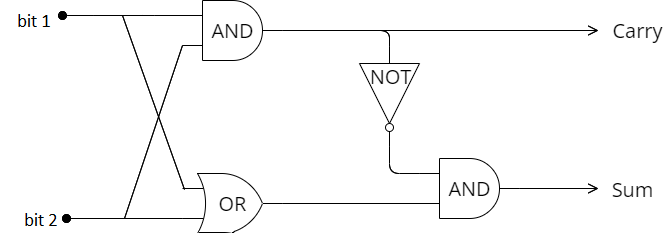
\includegraphics[width=0.5\textwidth]{files/half-adder.png}
    \end{center}
    \begin{enumerate}[(a)]
            \item Formalize this circuit in propositional logic. Specifically, express it as a theory $T=\{c\leftrightarrow \varphi,\ s\leftrightarrow \psi\}$ in the language $\mathbb P=\{b_1,b_2,c,s\}$, where the propositional variables mean ``bit 1'', ``bit 2'', ``carry'', and ``sum'', and the propositions $\varphi,\psi$ do not contain the variables $c,s$.
            \item Using the tableau method, prove that $T\models c\to\neg s$.
    \end{enumerate}

\end{problem}


\begin{problem}

    Using the compactness theorem, prove that every countable planar graph is four-colorable. You may use the Four Color Theorem (for finite graphs).

\end{problem}


        
\section*{For further thought}
        
        
\begin{problem}

    Prove directly (by transforming tableaux) the \emph{deduction theorem}, i.e., that for any theory $T$ and propositions $\varphi$, $\psi$, we have:
    $$
    T \proves \varphi\to\psi\text{\ \ if and only if\ \ }T,\varphi\proves  \psi
    $$

\end{problem}


\begin{problem}
    Let $A$ and $B$ be two non-empty theories in the same language. Suppose that every model of theory $A$ satisfies at least one axiom of theory $B$. Show that there exist finite sets of axioms $\{\alpha_1,\dots,\alpha_k\}\subseteq A$ and $\{\beta_1,\dots,\beta_n\}\subseteq B$ such that $\alpha_1\wedge\dots\wedge\alpha_k\,\to\,\beta_1\vee\dots\vee\beta_n$ is a tautology.
\end{problem}

